\section{Mitosis-Stream}\label{chap:mitosis-stream}
Mitosis-Stream is extending the Mitosis-Core with streaming functionality. While Mitosis-Core is responsible to set up an overlay network the Mitosis-Stream module is responsible to set up a \glsfirst{dag} to deliver video streams. The \gls{dag} is created over the existing overlay network.

\begin{figure}
\centering
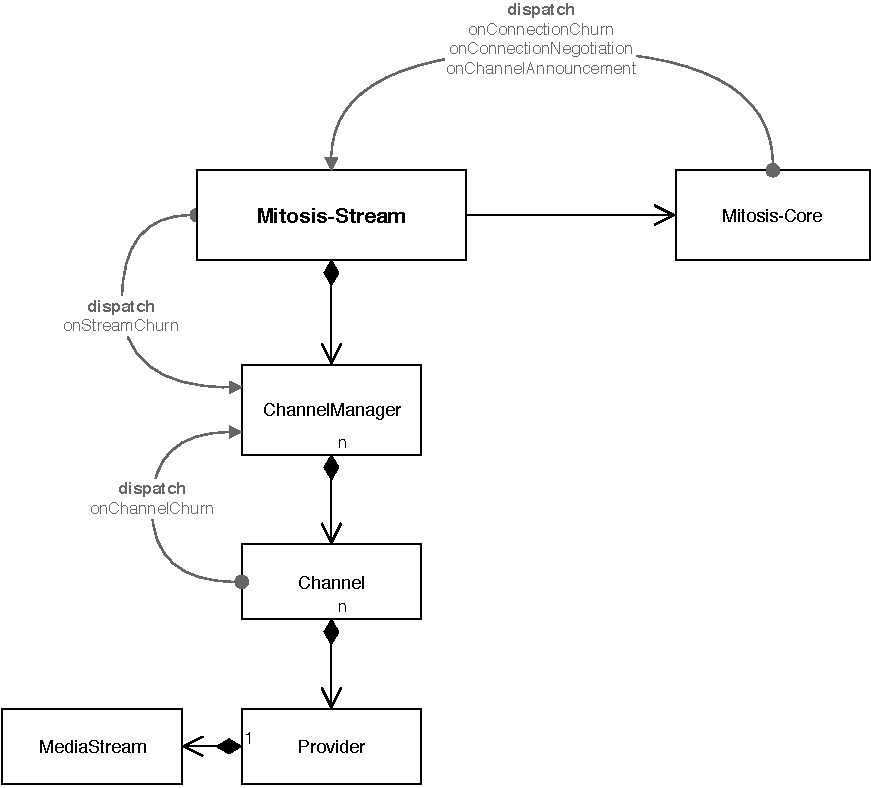
\includegraphics[width=0.75\textwidth]{graphics/implementation/mitosis-architecture-mitosis-stream.pdf}
\caption{Mitosis-Stream}
\label{fig:mit-stream}
\end{figure}

As presented in \vref{fig:mit-stream} Mitosis-Stream brings its own components and interacts with Mitosis-Core via the given interface. 

\subsection{ChannelManager}
The \lstinline|ChannelManger| is the owner of all available \lstinline|Channels|. Through the ChannelManager new Channels can be added.
There are three scenarios where a new Channel is added.
\begin{enumerate}
    \itembf{Peer creates one} The ChannelManager provides a method \lstinline|setLocalStream| and accepts a \lstinline|MediaStream| as argument. When the method is called the ChannelManager creates a new Channel and adds the peer as Provider.
    \itembf{Stream-Connection is opened} When a new stream connection is opened that the peer has not requested the ChannelManager creates a new channel and adds the stream connection initiator as provider.
    \itembf{ChannelAnnouncement} On receive of a \channelAnnouncement a new Channel is added with the peer who is announcing the channel as provider. When the channel has been created already the announcing peer is added as provider.
\end{enumerate}

\subsection{Channel}
A Channel is the representation of a broadcast. As the broadcast can be received by multiple peers, each peer providing a broadcast is represented as provider. A provider is active when the peer has an open WebRTCStream connection and actively receives a \lstinline|MediaStream|. Each provider has a maximum of allowed WebRTCStream connections. The maximum is represented as capacity. For example when a peer can open two more WebRTCStream connections it has a capacity of $\ 2 $.